\clearpage
\item \points{15} {\bf Logistic Regression: Training stability}

In this problem, we will be delving deeper into the workings of logistic
regression. The goal of this problem is to help you develop your skills
debugging machine learning algorithms (which can be very different from
debugging software in general).

We have provided a implementation of logistic regression in
\texttt{src/p01\_lr.py}, and two labeled datasets $A$ and $B$ in
\texttt{data/ds1\_a.txt} and \texttt{data/ds1\_b.txt}

Please do not modify the code for the logistic regression training algorithm
for this problem. First, run the given logistic regression code to train two
different models on $A$ and $B$. You can run the code by simply executing 
\texttt{python p01\_lr.py} in the \texttt{src} directory.

\begin{enumerate}

  \item \subquestionpoints{2}
What is the most notable difference in training the logistic regression model
on datasets $A$ and $B$?

\ifnum\solutions=1 {
  \begin{answer}
	\\
	Training the logistic regression model on dataset $B$ takes a very long time, comparing to the training process on dataset $A$.
\end{answer}

} \fi


  \item \subquestionpoints{5}
Investigate why the training procedure behaves unexpectedly on dataset $B$, but
not on $A$. Provide hard evidence (in the form of math, code, plots, etc.) to
corroborate your hypothesis for the misbehavior. Remember, you should address
why your explanation does \emph{not} apply to $A$.

\textbf{Hint}: The issue is not a numerical rounding or over/underflow error.

\ifnum\solutions=1 {
  \begin{answer}
	\\
	First, plot two datasets and we can discover that dataset $B$ is linear separable while dataset $A$ is not.
	
	\begin{figure}[h]
		\centering
		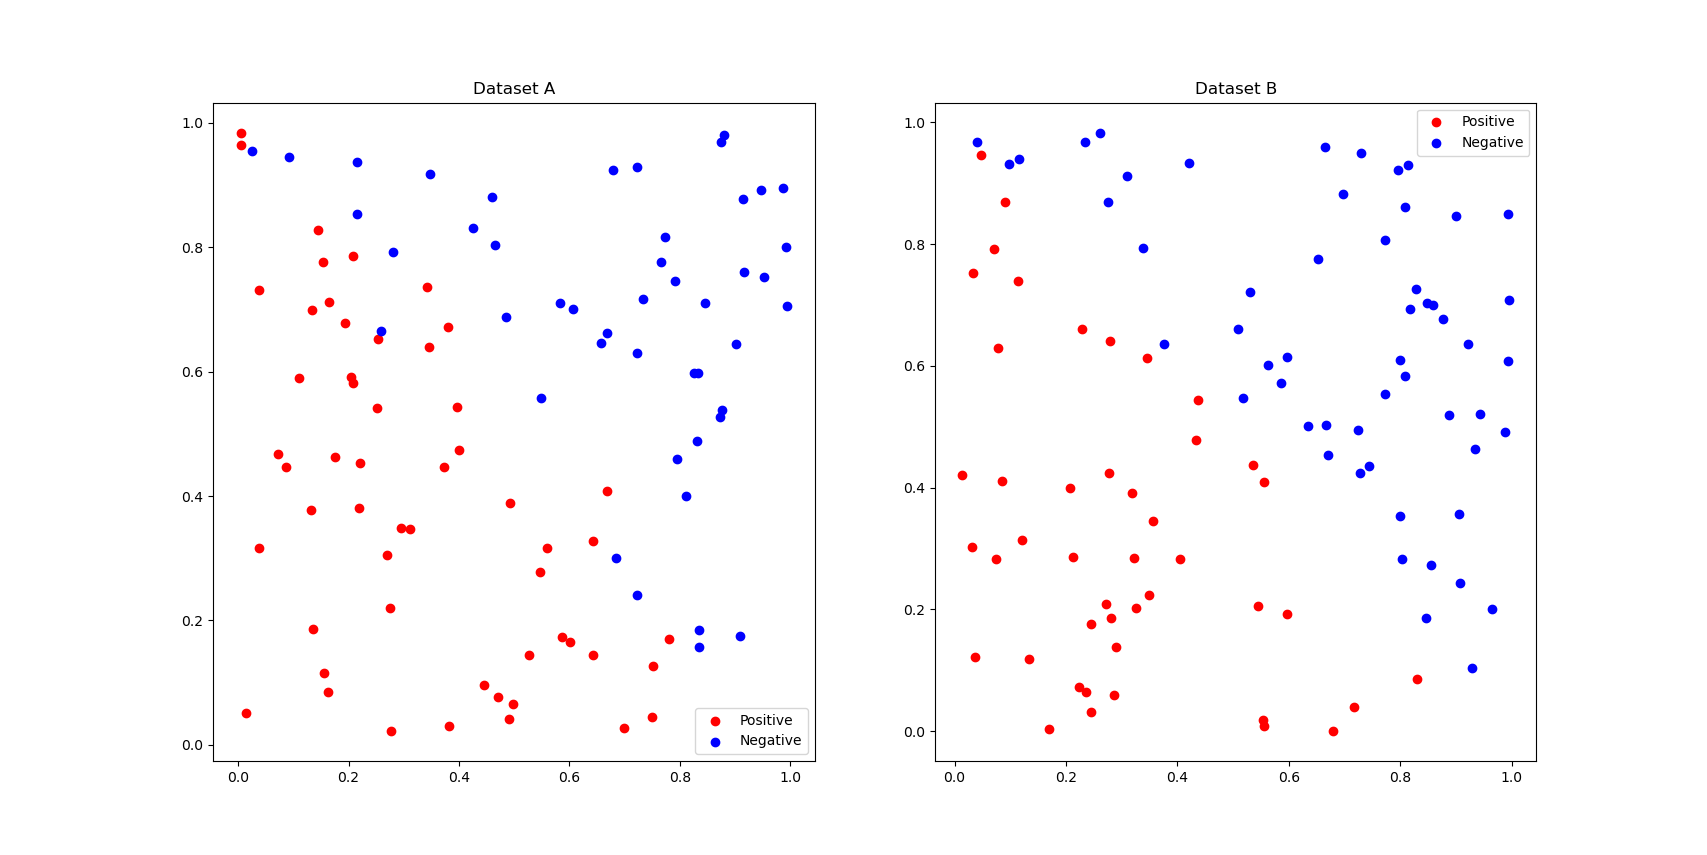
\includegraphics[width=0.7\linewidth]{01-stability/assets/datasets}
		\caption{}
		\label{fig:datasets}
	\end{figure}
	
	By observing the code, we find the gradient of loss function $J(\theta)$ is
	
	$$
	\nabla_{\theta} J(\theta) = -\frac{1}{m}\sum_{i = 1}^m \frac{x^{(i)}y^{(i)}}{1 + \exp(y^{(i)} \theta^T x^{(i)})}\\
	$$
	
	So we can infer what $J(\theta)$ is:
	
	$$
	J(\theta) = -\frac{1}{m}\sum_{i=1}^{m} \ln\frac{1}{1 + \exp(-y^{(i)} \theta^T x^{(i)})}
	$$
	
	For dataset $B$, which is linear separable, all examples within $B$ satisfies $y^{(i)}\theta^T x^{(i)}>0$, while there exists some examples within $A$ that satisfies $y^{(i)}\theta^T x^{(i)}<0$, since $A$ is not linear separable.
	
	For those examples $(x^{(i)}, y^{(i)})$ in $A$ that can't be classified correctly with a certain $\theta$, adjusting $\theta$ to make those examples well classified requires breaking the current situation where the hypothesis performs well on most examples and making $J(\theta)$ bigger. So the algorithm will leave $J(\theta)$ approximately unchanged by returning a gradient of a small norm, in other words, $J(\theta)$ converges.
	
	In contrast, there always exists a way to decrease $J(\theta)$ of dataset $B$, so $J(\theta)$ will keep decreasing rather than converge until it is truly very closed to the minimum.
\end{answer}

} \fi


  \item \subquestionpoints{5}
For each of these possible modifications, state whether or not it would lead to
the provided training algorithm converging on datasets such as $B$. Justify your
answers.
\begin{enumerate}
  \item Using a different constant learning rate.
  \item Decreasing the learning rate over time (e.g. scaling the initial
  learning rate by $1/t^2$, where $t$ is the number of gradient descent
  iterations thus far).
  \item Linear scaling of the input features.
  \item Adding a regularization term $\|\theta\|_2^2$ to the loss function.
  \item Adding zero-mean Gaussian noise to the training data or labels.
\end{enumerate}
 
\ifnum\solutions=1 {
  \begin{answer}
	\begin{enumerate}
		\item
		No. Because the gradient decreases very slowly with a relatively large initial value, which means that it will take a long time before $\Delta\theta$ approaches to $10^{-15}$. To make $\theta$ converge faster by making $\Delta\theta$ small at first, a rather small learning rate should be used. But a small and unchanged learning rate will contributes to small change of $\theta$, far from a right $\theta$. In other word, this will lead to a underfit model.
		
		\item
		Yes. By using this technique, $\Delta\theta$ will be limited by the number of iterations.
		
		\item 
		No. Linear scaling will not change the relative positions of each examples, thus will not change the fact whether the dataset is linear separable or not.
		
		\item 
		$\|\theta\|_2^2$ stops the original $J(\theta)$ decreasing continuous with $\theta$ changing.
		
		\item
		According to the explanation in (b), adding zero-mean Gaussian noise can make the dataset linear inseparable and the training procedure converges faster.
	\end{enumerate}
\end{answer}

} \fi

 
  
  \item \subquestionpoints{3} Are support vector machines, which use the hinge
loss, vulnerable to datasets like $B$? Why or why not? Give an informal
justification.

\ifnum\solutions=1 {
  \begin{answer}
	When training SVM on linear separable dataset, hinge loss is zero, and then the algorithm stops.
\end{answer}

} \fi


\end{enumerate}

\textbf{Hint:} Recall the distinction between functional margin and geometric
margin.
